\begin{figure}[t!]
  \centering
    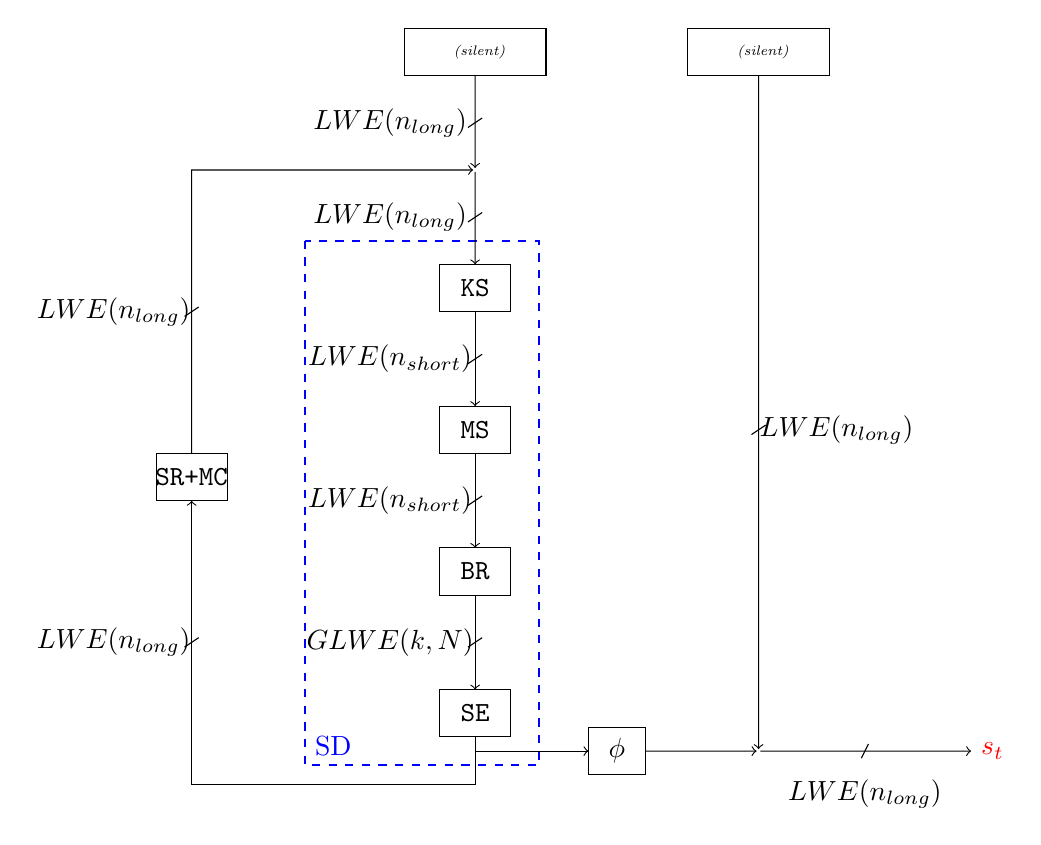
\begin{tikzpicture}[xscale=0.9,yscale=0.6]
 
    %LSFRs
    \draw[] (0, 0) rectangle (2, 1) node[pos=0.5]{$\pseudoKS$ {\tiny \emph{(silent)}}} ;
    \draw[] (4, 0) rectangle (6, 1) node[pos=0.5]{$\whitening$ {\tiny \emph{(silent)}}} ;
    \draw (1, -2) node[inner sep=0pt](addm){$\boxplus$} ;
    \draw[->] (1, 0) -- (addm);

    % FSM
    \draw[] (0.5, -4) rectangle (1.5, -5) node[pos=0.5,color=black](ks){$\texttt{KS}$} ;
    \draw[] (0.5, -7) rectangle (1.5, -8) node[pos=0.5,color=black](ms){$\texttt{MS}$} ;
    \draw[] (0.5, -10) rectangle (1.5, -11) node[pos=0.5,color=black](br){$\texttt{BR}$} ;
    \draw[] (0.5, -13) rectangle (1.5, -14) node[pos=0.5,color=black](se){$\texttt{SE}$} ;
    \draw[] (-3.5, -8) rectangle (-2.5, -9) node[pos=0.5,color=black](srmc){$\texttt{SR+MC}$} ;

    % Draw dashed blue box for SB
    \draw[dashed, blue, thick] (-1.4, -3.5) rectangle (1.9, -14.6);
    \node[blue] at (-1, -14.2) {SD}; % Label for the box

    % FSM connections
    \draw[->] (addm) -- (1, -4);
    \draw[->] (1, -5) -- (1, -7);
    \draw[->] (1, -8) -- (1, -10);
    \draw[->] (1, -11) -- (1, -13);
    \draw[->] (1,-14) -- (1, -15) -- (-3, -15) -- (-3, -9);
    \draw[->] (-3, -8) -- (-3, -2) -- (addm);

    % Extraction
    \draw (5, -14.3) node[inner sep=0pt](addr){$\boxplus$} ;
    \draw[] (2.6, -13.8) rectangle (3.4, -14.8) node[pos=0.5,color=black]{$\phi$} ;

    \draw[->] (1, -14.3) -- (2.6, -14.3);
    \draw[->] (3.4, -14.3) -- (addr);
    \draw[->] (5, 0) -- (addr);
    \draw[->] (addr) -- (8, -14.3);
    \draw[color=red] (8.3, -14.3) node(s){$s_t$} ;



    % Wire type
    \draw (0.9, -1.1) -- (1.1, -0.9) ;
    \draw (-0.2, -1) node{$LWE(n_{\text{long}})$} ;
    \draw (0.9, -3.1) -- (1.1, -2.9) ;
    \draw (-0.2, -3) node{$LWE(n_{\text{long}})$} ;
    \draw (0.9, -6.1) -- (1.1, -5.9) ;
    \draw (-0.2, -6) node{$LWE(n_{\text{short}})$} ;
    \draw (0.9, -9.1) -- (1.1, -8.9) ;
    \draw (-0.2, -9) node{$LWE(n_{\text{short}})$} ;
    \draw (0.9, -12.1) -- (1.1, -11.9) ;
    \draw (-0.2, -12) node{$GLWE(k, N)$} ;
    \draw (-3.1, -12.1) -- (-2.9, -11.9) ;
    \draw (-4.1, -12) node{$LWE(n_{\text{long}})$} ;
    \draw (-3.1, -5.1) -- (-2.9, -4.9) ;
    \draw (-4.1, -5) node{$LWE(n_{\text{long}})$} ;
    \draw (4.9, -7.6) -- (5.1, -7.4) ;
    \draw (6.1, -7.5) node{$LWE(n_{\text{long}})$} ;
    \draw (6.45, -14.45) -- (6.55, -14.15) ;
    \draw (6.5, -15.2) node{$LWE(n_{\text{long}})$} ;

    \end{tikzpicture}
  \vspace{1em}
  \hfill~
  \caption{\label{fig:structure_fhe} Types and shapes of ciphertexts in homomorphic \coolName. The $\subWords$ is broken down into its elementary components}
\end{figure}


% Leo: ce qui suit est pour qu'emacs compile bien l'article, pas touche !
%%% Local Variables:
%%% mode: latex
%%% ispell-local-dictionary: "english"
%%% TeX-master: "../main"
%%% End:



